\documentclass[12pt,a4paper]{article}

% ─── Page Layout ───────────────────────────────────────────────────────────────
\usepackage[a4paper, margin=0.8in, headheight=14pt]{geometry}

% ─── Fonts (XeLaTeX) ───────────────────────────────────────────────────────────
\usepackage{fontspec}
\usepackage{unicode-math}
\setmainfont{TeX Gyre Pagella}
\setmonofont[Scale=0.88]{TeX Gyre Cursor}
\setmathfont{Latin Modern Math}

% ─── Packages ──────────────────────────────────────────────────────────────────
\usepackage{xcolor}
\usepackage{colortbl}
\usepackage{titlesec}
\usepackage{enumitem}
\usepackage{tabularx}
\usepackage{booktabs}
\usepackage{array}
\usepackage{amsmath}
\usepackage{tikz}
\usetikzlibrary{shapes.geometric, arrows.meta, positioning, calc, fit, decorations.pathreplacing, patterns}
\usepackage{tcolorbox}
\tcbuselibrary{skins, breakable}
\usepackage{hyperref}
\usepackage{fancyhdr}
\usepackage{graphicx}
\usepackage{microtype}
\hyphenpenalty=10000
\exhyphenpenalty=10000
\sloppy
\usepackage{caption}
\usepackage{setspace}
\usepackage{multirow}
\usepackage{tocloft}

% ─── Q&A helper ────────────────────────────────────────────────────────────────
\newcommand{\Q}[1]{\textbf{#1}\par\noindent\ignorespaces}

% ─── Colour Palette ────────────────────────────────────────────────────────────
\definecolor{myred}{RGB}{196,30,58}
\definecolor{mydark}{RGB}{30,30,50}
\definecolor{mygreen}{RGB}{14,120,80}
\definecolor{myteal}{RGB}{0,130,140}
\definecolor{myamber}{RGB}{180,100,0}
\definecolor{mypurple}{RGB}{100,30,160}
\definecolor{mygray}{RGB}{246,247,249}
\definecolor{mgframe}{RGB}{180,185,200}
\definecolor{watermark}{RGB}{145,150,170}
\definecolor{hdrred}{RGB}{250,232,235}
\definecolor{hdrgreen}{RGB}{220,244,233}
\definecolor{hdrteal}{RGB}{220,242,244}
\definecolor{hdramber}{RGB}{253,242,215}
\definecolor{hdrpurple}{RGB}{238,228,255}
\definecolor{hdrgray}{RGB}{238,240,245}
\definecolor{rowalt}{RGB}{250,251,253}

% ─── Section Formatting ────────────────────────────────────────────────────────
\titleformat{\section}{\large\bfseries\color{myred}}{\thesection.}{0.5em}{}[\vspace{1pt}{\color{myred}\rule{\linewidth}{0.8pt}}]
\titleformat{\subsection}{\normalsize\bfseries\color{myteal}}{\thesubsection}{0.5em}{}
\titlespacing*{\section}{0pt}{18pt}{7pt}
\titlespacing*{\subsection}{0pt}{11pt}{4pt}

% ─── Paragraph ─────────────────────────────────────────────────────────────────
\setlength{\parindent}{0pt}
\setlength{\parskip}{4pt}

% ─── TOC Styling ───────────────────────────────────────────────────────────────
\renewcommand{\cfttoctitlefont}{\large\bfseries\color{myred}}
\renewcommand{\cftaftertoctitle}{\par\noindent{\color{myred}\rule{\linewidth}{0.8pt}}}
\setlength{\cftbeforetoctitleskip}{0pt}
\setlength{\cftaftertoctitleskip}{6pt}
\renewcommand{\cftsecfont}{\normalsize\bfseries\color{mydark}}
\renewcommand{\cftsecpagefont}{\normalsize\bfseries\color{mydark}}
\renewcommand{\cftsecleader}{\cftdotfill{\cftdotsep}}
\setlength{\cftbeforesecskip}{7pt}
\renewcommand{\cftsubsecfont}{\small\color{mydark}}
\renewcommand{\cftsubsecpagefont}{\small\color{mydark}}
\setlength{\cftbeforesubsecskip}{3pt}
\setlength{\cftsubsecindent}{1.4em}

% ─── Table helpers ─────────────────────────────────────────────────────────────
\renewcommand{\arraystretch}{1.45}
\setlength{\tabcolsep}{6pt}
\arrayrulecolor{mydark}
\newcolumntype{B}[1]{>{\small\bfseries\raggedright\arraybackslash}m{#1}}
\newcolumntype{Y}{>{\small\raggedright\arraybackslash}X}
\renewcommand{\tabularxcolumn}[1]{m{#1}}

% ─── Header / Footer ───────────────────────────────────────────────────────────
\pagestyle{fancy}
\fancyhf{}
\fancyhead[L]{\small\color{myred}\textbf{OE-EC803B}\;\color{mydark}--- Big Data Analysis}
\fancyhead[R]{\small\color{myteal}\textbf{Module 3 Notes}}
\fancyfoot[C]{\small\color{mydark}\thepage}
\fancyfoot[R]{\small\color{watermark}\textit{\copyright\ Biraj Sarkar}}
\renewcommand{\headrulewidth}{0.5pt}
\renewcommand{\footrulewidth}{0.3pt}

% ─── Hyperref ──────────────────────────────────────────────────────────────────
\hypersetup{colorlinks=true, linkcolor=myteal, urlcolor=myteal,
  pdfauthor={Biraj Sarkar}, pdftitle={OE-EC803B --- Module 3 Notes}}

% ─── tcolorbox styles ──────────────────────────────────────────────────────────
\tcbset{
  tikzbox/.style={colback=mygray, colframe=mgframe, boxrule=0.6pt, arc=4pt,
    left=8pt, right=8pt, top=6pt, bottom=6pt,
    colbacktitle=mgframe, coltitle=mydark, fonttitle=\small\bfseries, unbreakable},
  defbox/.style={colback=hdrgreen, colframe=mygreen, boxrule=0.8pt, arc=4pt,
    left=9pt, right=9pt, top=6pt, bottom=6pt,
    colbacktitle=mygreen, coltitle=white, fonttitle=\small\bfseries},
  formulabox/.style={colback=hdrteal, colframe=myteal, boxrule=0.8pt, arc=4pt,
    left=9pt, right=9pt, top=7pt, bottom=7pt,
    colbacktitle=myteal, coltitle=white, fonttitle=\small\bfseries},
  examplebox/.style={colback=hdramber, colframe=myamber, boxrule=0.8pt, arc=4pt,
    left=9pt, right=9pt, top=6pt, bottom=6pt,
    colbacktitle=myamber, coltitle=white, fonttitle=\small\bfseries},
  masonbox/.style={colback=hdrpurple, colframe=mypurple, boxrule=0.8pt, arc=4pt,
    left=9pt, right=9pt, top=6pt, bottom=6pt,
    colbacktitle=mypurple, coltitle=white, fonttitle=\small\bfseries},
  exambox/.style={colback=hdrpurple, colframe=mypurple, boxrule=1pt, arc=5pt,
    left=10pt, right=10pt, top=8pt, bottom=8pt,
    colbacktitle=mypurple, coltitle=white, fonttitle=\bfseries,
    breakable, title after break={\textbf{Frequently Asked / Viva Questions (contd.)}}}
}
\tcbset{breakable}

% ─── TikZ styles ───────────────────────────────────────────────────────────────
\tikzset{
  block/.style={rectangle, draw=myteal, fill=hdrteal,
    text width=2.2cm, align=center, minimum height=0.9cm,
    font=\small, rounded corners=3pt, line width=0.7pt},
  redblock/.style={rectangle, draw=myred, fill=hdrred,
    text width=2.2cm, align=center, minimum height=0.9cm,
    font=\small, rounded corners=3pt, line width=0.7pt},
  arrow/.style={-Stealth, thick, color=mydark},
  redarrow/.style={-Stealth, thick, color=myred},
  line/.style={thick, color=mydark}
}

\begin{document}

% ═══════════════════════════════════════════════════════════════════════════════
% TITLE BLOCK
% ═══════════════════════════════════════════════════════════════════════════════
\begin{center}
  \hfill \textit{Exam-Ready Short Notes} \\
  \vspace{6pt}
  {\LARGE\bfseries\color{myred} OE-EC803B --- Big Data Analysis}\\[5pt]
  {\normalsize\color{mydark} Semester VIII \quad$\bullet$\quad 3L:0T:0P \quad$\bullet$\quad 3 Credits}\\[3pt]
  {\normalsize\color{myteal}\textbf{Module 3: MapReduce Programming Paradigm \& YARN Resource Manager}}\\[3pt]
  {\small\color{mydark} CGEC \;$|$\; B.Tech ECE (2023--27) \;$|$\; \textit{Biraj Sarkar}}
\end{center}
\vspace{2pt}
\noindent{\color{myred}\rule{\linewidth}{1.5pt}}
\vspace{2pt}

\hypersetup{linkcolor=mydark}
\tableofcontents
\hypersetup{linkcolor=myteal}
\newpage

% ===============================================================================
\section{Anatomy of a MapReduce Job Run}
% ===============================================================================

MapReduce execution is divided into MapReduce 1 (Classic MapReduce) and MapReduce 2 (built on YARN).

\begin{tcolorbox}[defbox, title={Classic MapReduce vs. YARN}]
  \begin{itemize}[leftmargin=*, noitemsep]
    \item \textbf{MapReduce 1 (Classic):} Job execution was coordinated by a single master process called the \textbf{JobTracker}, which scheduled tasks and monitored slaves called \textbf{TaskTrackers}.
    \item \textbf{YARN (MapReduce 2):} Divides the resource management and job scheduling functions into separate daemons: a global \textbf{ResourceManager} and application-specific \textbf{ApplicationMasters}.
  \end{itemize}
\end{tcolorbox}

\subsection{YARN Runtime Job Execution Steps}
YARN runs MapReduce jobs using several steps:
\begin{enumerate}[leftmargin=*, itemsep=3pt]
  \item \textbf{Job Submission:} The Client program calls `submitJob()` on the Job object, requesting a new Application ID from the ResourceManager.
  \item \textbf{Application Master Launch:} The ResourceManager allocates a \textbf{Container} (allocated CPU/RAM limit) on a NodeManager and starts the \textbf{ApplicationMaster} process there.
  \item \textbf{Resource Allocation:} The ApplicationMaster registers with the ResourceManager and requests containers across NodeManagers to host the Map and Reduce tasks.
  \item \textbf{Task Execution:} The ApplicationMaster contacts the NodeManagers to launch the tasks within the allocated containers. Tasks retrieve data blocks from local HDFS DataNodes, process them, and write outputs locally.
\end{enumerate}

\begin{tcolorbox}[tikzbox, title={YARN Resource Management Layout}]
\centering
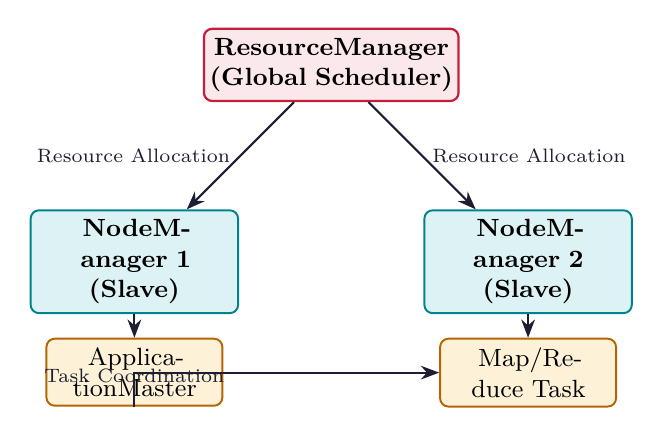
\begin{tikzpicture}[node distance=0.8cm and 1.2cm,
  rmnode/.style={rectangle, draw=myred, fill=hdrred, text width=3.0cm, align=center, minimum height=0.85cm, font=\small\bfseries, rounded corners=3pt, line width=0.8pt},
  nmnode/.style={rectangle, draw=myteal, fill=hdrteal, text width=2.4cm, align=center, minimum height=0.8cm, font=\small\bfseries, rounded corners=3pt, line width=0.7pt},
  cnode/.style={rectangle, draw=myamber, fill=hdramber, text width=2.0cm, align=center, minimum height=0.75cm, font=\small, rounded corners=3pt, line width=0.7pt},
  lnarrow/.style={-Stealth, thick, color=mydark}]

  % Nodes
  \node[rmnode] (rm) at (0,2.5) {ResourceManager\\(Global Scheduler)};
  \node[nmnode] (nm1) at (-2.5,0) {NodeManager 1\\(Slave)};
  \node[nmnode] (nm2) at (2.5,0) {NodeManager 2\\(Slave)};

  \node[cnode, below=0.3cm of nm1] (am) {ApplicationMaster};
  \node[cnode, below=0.3cm of nm2] (task) {Map/Reduce Task};

  % Connections
  \draw[lnarrow] (rm) -- node[left, font=\scriptsize] {Resource Allocation} (nm1);
  \draw[lnarrow] (rm) -- node[right, font=\scriptsize] {Resource Allocation} (nm2);
  \draw[lnarrow] (nm1) -- (am);
  \draw[lnarrow] (nm2) -- (task);
  \draw[lnarrow] (am) |- node[pos=0.2, above, font=\scriptsize] {Task Coordination} (task.west);

\end{tikzpicture}
\end{tcolorbox}

% ===============================================================================
\section{Failures in YARN}
% ===============================================================================

Distributed systems must tolerate node and task failures gracefully.

\subsection{Task Failure}
A Map or Reduce task can fail due to runtime Java exceptions or JVM crashes.
\begin{itemize}[leftmargin=*, itemsep=3pt]
  \item \textbf{Detection:} The NodeManager detects that the task JVM exited with a non-zero code and reports the failure back to the ApplicationMaster.
  \item \textbf{Resolution:} The ApplicationMaster reschedules the task on a different NodeManager. It will retry the task up to 4 times (default limit) before marking the entire job as failed.
\end{itemize}

\subsection{NodeManager Failure}
\begin{itemize}[leftmargin=*, itemsep=3pt]
  \item \textbf{Detection:} The NodeManager sends heartbeats to the ResourceManager. If heartbeats stop (typically for 10 minutes), the ResourceManager marks the NodeManager as dead.
  \item \textbf{Resolution:} The ResourceManager notifies the active ApplicationMasters. The ApplicationMasters reschedule all tasks (both active and completed map tasks) that were running on the failed NodeManager, since their local map outputs are no longer accessible.
\end{itemize}

\subsection{ResourceManager / ApplicationMaster Failure}
\begin{itemize}[leftmargin=*, itemsep=3pt]
  \item \textbf{ApplicationMaster Failure:} The ResourceManager detects the loss of heartbeat from the ApplicationMaster and starts a new container to launch a fresh ApplicationMaster instance.
  \item \textbf{ResourceManager Failure:} This is a single point of failure (SPOF). It is resolved by running active-standby ResourceManagers using ZooKeeper to manage failover and state replication.
\end{itemize}

% ===============================================================================
\section{Job Scheduling}
% ===============================================================================

YARN supports three primary job scheduling engines:

\begin{enumerate}[leftmargin=*, itemsep=4pt]
  \item \textbf{FIFO (First-In, First-Out) Scheduler:} Allocates resources strictly based on job submission order. A large, slow job at the head of the queue will block all subsequent small jobs.
  \item \textbf{Capacity Scheduler:} Allocates distinct organizational queues, where each queue is guaranteed a fixed percentage of cluster capacity (e.g., Queue A gets 40\%, Queue B gets 60\%). If a queue has free space, it can temporarily lend it to other queues.
  \item \textbf{Fair Scheduler:} Dynamically balances resources so that all running jobs get an equal share of cluster capacity over time. When a single job runs, it uses 100\% of the cluster; when a second job is submitted, YARN re-allocates 50\% of the resources to it.
\end{enumerate}

% ===============================================================================
\section{Shuffle and Sort Phase}
% ===============================================================================

\begin{tcolorbox}[defbox, title={The Shuffle and Sort}]
  The \textbf{Shuffle and Sort} is the core transport layer of MapReduce that routes intermediate key-value outputs from mappers to the correct reducers, guaranteeing that all values associated with a specific key are grouped and delivered to the same reducer in sorted order.
\end{tcolorbox}

The shuffle process runs across the map and reduce stages:

\subsection{Map Side Execution Details}
\begin{enumerate}[leftmargin=*, itemsep=3pt]
  \item \textbf{Circular Buffer:} The Map task writes outputs to an in-memory circular RAM buffer (default size: 100MB).
  \item \textbf{Spilling:} When the buffer fill percentage reaches a threshold (default: 80\%), a background thread wakes up to spill the data to the local disk.
  \item \textbf{Partitioning:} Before writing to disk, the thread divides the key-value records into partitions based on the target Reducer ID (using \texttt{HashPartitioner} by default: \texttt{(key.hashCode() \& Integer.MAX\_VALUE) \% numReducers}).
  \item \textbf{Sorting:} Within each partition, the keys are sorted in memory using a quicksort algorithm.
  \item \textbf{Combining:} If a local `Combiner` (mini-reducer) is defined, it runs on the sorted partition records before writing to disk to reduce data volume.
  \item \textbf{Merging:} When the Map task finishes, all local spill files are merged and sorted to create a single partitioned and sorted output file on the local node.
\end{enumerate}

\subsection{Reduce Side Execution Details}
\begin{enumerate}[leftmargin=*, itemsep=3pt]
  \item \textbf{Copy Phase:} The Reducer tasks have copier threads that fetch their respective partition files from all mapper nodes over HTTP (using the MapOutputServlet).
  \item \textbf{Merge Phase:} As files are copied, background threads merge and sort the incoming data in passes.
  \item \textbf{Reduce Phase:} The sorted key-value pairs are fed to the `reduce()` method line-by-line.
\end{enumerate}

% ===============================================================================
\section{MapReduce Types and Formats}
% ===============================================================================

MapReduce enforces strict type checking using serialization wrappers (e.g., `Text` for Java String, `IntWritable` for Integer).

\subsection{Input Splits and InputFormat}
\begin{itemize}[leftmargin=*, itemsep=3pt]
  \item \textbf{InputSplit:} A chunk of HDFS data processed by a single mapper. Typically equals the HDFS block size (128MB).
  \item \textbf{InputFormat:} Validates the input files and defines how to split them. It spawns the \textbf{RecordReader} to convert split byte streams into key-value records.
\end{itemize}

\par\vspace{6pt}\noindent
{\renewcommand{\arraystretch}{1.4}%
\begin{tabularx}{\linewidth}{|B{3.2cm}|Y|Y|}
\hline
\textbf{InputFormat} & \textbf{Key Type} & \textbf{Value Type} \\
\hline
`TextInputFormat` & `LongWritable` (Byte offset of line) & `Text` (Content of the text line) \\
\hline
`KeyValueTextInputFormat` & `Text` (Text before separator) & `Text` (Text after separator) \\
\hline
`SequenceFileInputFormat` & User-defined binary key type & User-defined binary value type \\
\hline
\end{tabularx}}

% ===============================================================================
\section{Advanced MapReduce Features}
% ===============================================================================

\subsection{Counters}
Counters are used to collect statistics about MapReduce jobs (e.g., counting empty records or corrupt lines).
\begin{itemize}[leftmargin=*, itemsep=3pt]
  \item \textbf{Built-in Counters:} Automatically populated by YARN (e.g., Map Input Records, Bytes Written).
  \item \textbf{User-Defined Counters:} Programmed in Java using enums: \texttt{context.getCounter(MyEnum.CORRUPT\_ROWS).increment(1)}.
\end{itemize}

\subsection{Joins in MapReduce}
When combining datasets (e.g., Customers and Orders tables), two join strategies are used:

\par\vspace{6pt}\noindent
{\renewcommand{\arraystretch}{1.4}%
\begin{tabularx}{\linewidth}{|B{3.0cm}|Y|Y|}
\hline
\textbf{Feature} & \textbf{Map-Side Join} & \textbf{Reduce-Side Join} \\
\hline
Execution Phase & Done completely inside the Mapper. & Done inside the Reducer. \\
\hline
Prerequisites & Datasets must be sorted and bucketed by the join key. One dataset must be small enough to fit in memory. & None. General-purpose join. \\
\hline
Shuffle Overhead & Zero shuffle overhead (fastest). & Heavy network shuffle of all records. \\
\hline
Data Volume Limit & Limited by Mapper node RAM. & Unlimited (handles massive datasets). \\
\hline
\end{tabularx}}

\newpage

% ═══════════════════════════════════════════════════════════════════════════════
% QUICK REVISION PAGE
% ═══════════════════════════════════════════════════════════════════════════════
\begin{center}
  {\large\bfseries\color{myred} Quick Revision --- Module 3}\\[3pt]
  {\small\color{mydark} MapReduce Internals, YARN Scheduler \& Joins $|$ OE-EC803B}
\end{center}
\noindent{\color{myred}\rule{\linewidth}{1.2pt}}
\vspace{8pt}

\begin{tcolorbox}[defbox, title={\textbf{One-Line Definitions}}]
\begin{itemize}[leftmargin=*, itemsep=3pt, topsep=0pt]
  \item \textbf{ApplicationMaster:} A per-application YARN process that negotiates resources and coordinates task runs.
  \item \textbf{Container:} A logical YARN resource allocation containing CPU cores and RAM limits on a NodeManager.
  \item \textbf{Speculative Execution:} A task execution strategy that runs duplicate copies of slow-running tasks in parallel to minimize job latency.
  \item \textbf{Combiner:} A local semi-reducer that aggregates Map outputs locally before the network shuffle.
  \item \textbf{RecordReader:} A helper class that translates raw HDFS data splits into structured key-value objects.
\end{itemize}
\end{tcolorbox}

\vspace{6pt}

\begin{tcolorbox}[exambox, title={\textbf{Frequently Asked / Viva Questions}}]
\begin{enumerate}[leftmargin=*, topsep=0pt, label=\textbf{Q\arabic*.}, itemsep=5pt]
  \item \Q{What are the differences between MapReduce 1 (Classic) and YARN?}
        In MapReduce 1, the JobTracker was responsible for both resource management and task scheduling, creating scalability bottlenecks. YARN decouples these tasks, using a global \textbf{ResourceManager} for cluster resource allocation and a per-job \textbf{ApplicationMaster} for scheduling.
        
  \item \Q{Detail the spilling process on the Map side.}
        Mappers write outputs to a 100MB circular buffer. When the buffer is 80\% full, a background thread locks the data, partitions it based on Reducer IDs, sorts it by key, runs the optional combiner, and writes (spills) the sorted partition files to local disk.
        
  \item \Q{How does the Fair Scheduler distribute cluster resources?}
        The Fair Scheduler divides resources dynamically so that all active jobs receive an equal share of CPU and RAM over time. If only one job runs, it uses the entire cluster. When a second job starts, YARN re-allocates 50\% of the resources to it.
        
  \item \Q{Why does a NodeManager failure force mappers to rerun, but not reducers?}
        Mappers store their intermediate partition outputs on local disks, so if the mapper's node dies, those files are lost. Reducers write their final outputs directly to replicated HDFS blocks, which remain accessible even if a NodeManager fails.
        
  \item \Q{What is the difference between TextInputFormat and KeyValueTextInputFormat?}
        `TextInputFormat` treats the line offset as the key (`LongWritable`) and the line text as the value (`Text`). `KeyValueTextInputFormat` splits each line at a separator character (like a tab) to define both the key and the value as `Text`.
        
  \item \Q{Explain Map-side Joins and their memory constraints.}
        A Map-side Join joins datasets inside the Mapper without a network shuffle. It requires that all datasets are pre-sorted and bucketed by the join key, and one of the datasets must be small enough to load entirely into the mapper's JVM memory.
        
  \item \Q{Why does speculative execution not run for tasks with side effects?}
        Speculative execution launches duplicate tasks. If a task writes to an external database, running duplicate tasks would cause duplicate writes. Therefore, speculative execution should be disabled for tasks with external side effects.
        
  \item \Q{What is the purpose of sync markers in a SequenceFile?}
        Sync markers are special byte sequences placed periodically in a SequenceFile. They allow MapReduce to split the file at arbitrary boundaries, as the RecordReader can seek to a random position and scan forward to find the next sync marker.
        
  \item \Q{How does secondary sorting work in MapReduce?}
        It allows sorting the values associated with a key. It is implemented by creating a composite key (comprising the natural key and the secondary sort value), partitioning by the natural key, and sorting by the composite key.
        
  \item \Q{What does the HashPartitioner do?}
        It computes the partition index for a mapper output key: \texttt{(key.hashCode() \& Integer.MAX\_VALUE) \% numReducers}. This ensures that all records with the same key are routed to the same Reducer ID.
\end{enumerate}
\end{tcolorbox}

\vspace{6pt}

\begin{tcolorbox}[tikzbox, title={\textbf{Comparison Snapshot}}]
\textbf{Capacity Scheduler vs. Fair Scheduler:}\par\vspace{6pt}\noindent
{\renewcommand{\arraystretch}{1.4}%
\begin{tabularx}{\linewidth}{|B{3.2cm}|Y|Y|}
\hline
\textbf{Feature} & \textbf{Capacity Scheduler} & \textbf{Fair Scheduler} \\
\hline
Primary Design Goal & Organization queues with guaranteed shares & Dynamic, equal sharing of cluster resources \\
\hline
Queue Configuration & Strict hierarchical queues (e.g., Sales, Dev) & Simple resource shares per running application \\
\hline
Resource Loaning & Queues can borrow unused capacity from others & Idle capacity is divided among active jobs \\
\hline
Preemption & Not supported (waits for tasks to end) & Supported (reclaims resources by killing tasks) \\
\hline
Use Case & Multi-tenant corporate cluster with fixed budgets & Ad-hoc environments with variable workloads \\
\hline
\end{tabularx}}
\end{tcolorbox}

\end{document}
